% !TEX root = ../lifeonbrane3.tex
%





%\subsection{`Bubbles' on the brane}\label{bubblesX}


In this closing section, we consider a simple but surprising class of RT surfaces. In particular, we show below that there are closed extremal surfaces with the topology of a sphere, \ie $S^{d-1}$ in the locally AdS$_{d+1}$ bulk geometry. In empty AdS space, one could consider such spherical surfaces, but their area would be extremized when they collapse to zero size. In the present case, we will show that in certain situations, the spherical RT surfaces can be supported at finite size by the brane.  To illustrate the situation, we continue with the special case of $d=3$ as in the previous section, and afterwards comment on the situation with general $d$. 
%
\begin{figure}[h]
\begin{center}
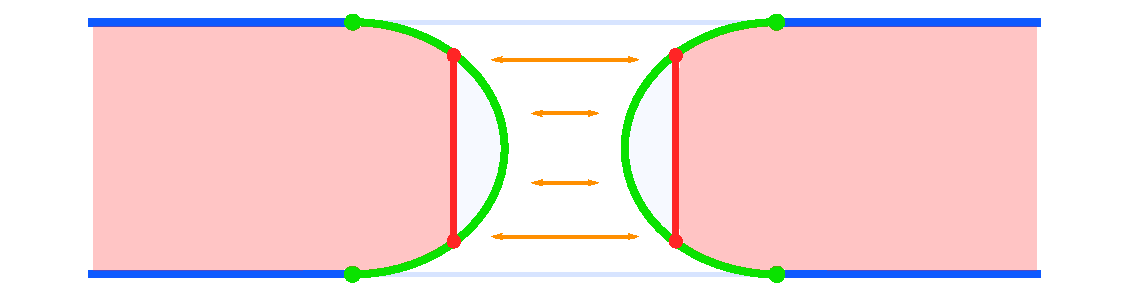
\includegraphics[scale=0.2]{images/bubble}
\caption{One half of an RT bubble supported on the brane. \rcm{Lets illustrate this in the `style' of figure \ref{fig:EWs}.}}
\label{figbubble}
\end{center}
\end{figure}

Consider the geometry illustrated in figure \ref{figbubble}. On either side of the brane, we have a disk satisfying $\zeta=$constant, \ie satisfying eq.~\reef{zetap} with $P_0=0$. Hence locally these surfaces extremize the entropy functional \reef{area} in the bulk. However, rather than extending out to the asymptotic boundary, as shown in the figure, the two disks intersect the brane and meet at some radius $\pb$.  Hence this RT surface has the topology of a sphere and we use the nomenclature `bubble' to describe these surfaces. For $d=3$, the generalised entropy \reef{eq:sad} of this bubble is
\begin{align}\label{Agenbubble}
\sgen&=\frac{\pi L^2}{\Gbk} \left(  \sqrt{1+\pb^2}-1  + \lamb\, \pb \right) +2\,\lgb 
\end{align}
with $\lamb$ defined in eq. \eqref{newdefs}. We have also included the topological term introduced in eq.~\reef{Euler3}.
%It also illuminating to contrast this with the formula for the effective gravitational constant on the brane, eq.~\eqref{Newton33}, which can be rewritten in terms of $\lambda$ as
%\begin{align}\label{Gefflambda}
%\Geff=\frac{\lambda}{1+\lambda}\Gbr
%\end{align}
%\rcm{see instead eq.~\reef{Newton34}.}

Extremizing eq.~\reef{Agenbubble} with respect to the radius of the bubble, we find
\beq\label{gamdot}
\partial_{\pb}\sgen=0 \qquad
\implies\qquad \frac{\pb}{\sqrt{1+\pb^2}}=-\lamb=-\frac{\Gbk}{2L\,\Gbr}\,.
\eeq
Now recall that we will always have $\Gbk>0$, but considered the possibility of $\Gbr$ becoming negative in the previous section. But let us first consider the case $\lamb\ge 0$, which implies $1/\Gbr\ge 0$. In this case, we can not satisfy eq.~\reef{gamdot} or rather both the bulk and brane contributions to the generalised entropy \eqref{Agenbubble} are positive monotonically increasing functions of $\pb$, and therefore the minimum lies at $\pb=0$, \ie where the bubble collapses to zero size -- see figure \reef{figAbubble}. 

Further, we might comment that for large $\pb$, the leading contribution in eq.~\reef{Agenbubble} takes the expected form
\beq\label{expect4}
\sgen\simeq =\frac{A(\sigma_\xR)}{4G_\mt{eff}} +\cdots \qquad{\rm where}\ \ \ \frac{A(\sigma_\xR)}{4G_\mt{eff}}=\frac{\pi L^2}{\Gbk}\,(1+\lamb)\,\pb\,,
\eeq
just as in eq.~\reef{radishes}. That is, \rcm{******}


Of course, the more interesting scenario is when $\lamb$, and hence
$1/\Gbr$, are negative. Then eq.~\reef{gamdot} has the solution
\begin{align}
\pbo=-\frac{\lamb}{\sqrt{1-\lamb^2}}\,,
\label{cookie}
\end{align}
for which the generalized entropy \reef{Agenbubble} becomes
\begin{align}\label{Sbubble}
\sgen= \frac{\pi L^2}{\Gbk} \left( \sqrt{1-\lamb^2} - 1 \right)+2\,\lgb 
\end{align}
We note that these expressions are only sensible for $-1<\lamb<0$. In fact, for $\lamb<-1$, there is no minimum for the generalized entropy \reef{Agenbubble}, \ie there is no solution for eq.~\reef{gamdot}, and rather $\pb$ runs off to infinity -- see figure \reef{figAbubble}.  This is, perhaps, not so surprising since we can see from eq.~\reef{Newton34} that this regime is pathological, with the graviton localized on the brane becoming a ghost.

Therefore we only consider the regime $-1<\lamb<0$ where eqs.~\reef{cookie} and \reef{Sbubble} apply. As illustrated in figure \reef{figAbubble}, eq.~\reef{cookie} is indeed the global minimum of the generalized entropy \eqref{Agenbubble}. We might note that the sum of the first two terms in eq.~\reef{Sbubble} is negative. That is, the combined contributions of the two area terms in eq.~\reef{eq:sad} is in fact {\it negative!} Hence we only get a sensible (\ie positive) result for the generalized entropy \reef{Agenbubble} with the inclusion of the topological term \reef{Euler3}, which was also favoured in section \ref{sec:examples}.


\begin{figure}[h]
\begin{center}
\includegraphics[scale=0.4]{images/Abubble}
\caption{The generalised area \eqref{Agenbubble} for a bubble as a function of its radius. For $\lambda>0$, the area is minimal for vanishing size, whereas for $-1<\lambda<0$ it has a finite size. For $\lambda<-1$, there is no global minimum, signalling an instability of the system. }
\label{figAbubble}
\end{center}
\end{figure}

\begin{align}\label{genbubble1}
S_\mt{gen}=\frac{L^{d-1}\,\Omega_{d-2}  }{2(d-1)\Gbk}\,P^{d-1}\, {}_{2}F_1\left[ \frac{1}{2},\frac{d-1}{2},\frac{d+1}{2},-P^2 \right]+\frac{L^{d-2}\, \Omega_{d-2}}{4\Gbr}\,P^{d-2}
\end{align}
\vc{From
\begin{align}
  \hyperF\left(
  \frac{1}{2},
  \frac{d-1}{2},
  \frac{d+1}{2},
  -P^2
  \right)
  \sim\begin{cases}
  1 & \text{if $P\ll 1$}
  \\
  \frac{d-1}{d-2}\frac{1}{P} &\text{if $P\gg 1$}
\end{cases}
\label{eq:bubblegum}
\end{align}
we see that the bulk contribution, for small $P$, is extensive, and for large $P$, is dominated by a term identical to the QES area term in \eqref{genbubble1} with $1/G_\brane$ replaced by the induced $1/G_\eff |_{1/G_\brane=0}$ given in \eqref{Newton2}. Note that performing a large $P$ expansion in the hypergeometric function \eqref{eq:bubblegum} is equivalent to the process of extracting the `divergent' entropy piece described around \eqref{eq:apple} --- in \eqref{genbubble1}, $G_\bulk$ is written in terms of $c\sim L^{d-1}/G_\bulk$ and $P$ is rescaled by $L$ to obtain a dimensionful coordinate, then a small $L$ expansion is performed. However, the extremal condition $\partial_P S_\gen =0$ can in fact be solved exactly for any $d$ as
\beq\label{amazing}
  \partial_P S_\gen
  = \frac{L^{d-1}\Omega_{d-2}}{2 G_\bulk} P^{d-3}\left(
  \frac{P}{\sqrt{P^2+1}} + \lambda
  \right)
\eeq
with the parenthesized factor vanishing at the radius \eqref{eq:cookie}.
}


To gain an intuitive understanding of bubbles from the brane's perspective, it is helpful to rewrite \eqref{Agenbubble} in the following suggestive form:
\begin{align}
  S_\gen
  =& \frac{\area}{4 G_\eff} + S_\ren.
  \label{eq:pear}
\end{align}
Here,
\begin{align}
  \frac{\area}{4 G_\eff}
  =& \frac{\area}{4 G_\brane} + S_\dive
\end{align}
is a sum of the bare area term (scaled by the bare Newton's constant of the brane),
\begin{align}
  \frac{\area}{4 G_\brane}
  =& \frac{\pi L P}{2 G_\brane}
  = \frac{\pi L^2 \lambda P}{G_\bulk}
  \label{eq:cucumber}
\end{align}
and the `divergent' part
\begin{align}
  S_\dive
  =& \frac{c \area}{L}
  = \frac{\pi L^2 P}{G_\bulk},
  &
  c \equiv& \frac{L^2}{2 G_\bulk}
  \label{eq:apple}
\end{align}
of the CFT entropy
\begin{align}
  S_\CFT
  =& S_\dive + S_\ren
  \label{eq:banana}
  \\
  S_\ren
  =& 2\pi c(\sqrt{1+P^2}-1-P)
  = \frac{\pi L^2(\sqrt{1+P^2}-1-P)}{G_\bulk}.
  \label{eq:orange}
\end{align}
To identify the terms introduced here, we first subtracted the bare area term \eqref{eq:cucumber} from \eqref{Agenbubble}, leaving the bulk area of the RT surface. We identify the latter as the entropy \eqref{eq:banana} of the matter CFT. To separate out the `divergent' contribution \eqref{eq:apple}, we invoke the usual holographic proportionality $G_\bulk \propto L^{d-1}/c$ (here $d=3$) between the bulk Newton's constant and the CFT central charge, temporarily remove $P$ in favour of a dimensionful coordinate $\tilde{P}\equiv P L$, and expand in $L$. This is because the displacement of the brane from the AdS boundary sets a UV cutoff in the brane theory at a proper length scale of $L$ (as measured by the induced metric). For $d>3$, divergent terms other than the area term are also expected to make an appearance. We collect the remaining `finite' contribution to the CFT entropy in $S_\ren$ given in \eqref{eq:orange}.


\subsection{Wormholes and Cutoffs}\label{wormy}

\rcm{old words:} These bubbles are a remnant of replica wormholes in the limit $n\to1$. What are lessons that we learn? Note that it is important that the wormholes depend on the quantum contributions of the matter fields. Hence they do not exist on their own, \ie they need to be anchored by a twist operator on the boundary.
What are the implications for the new discussions of baby universes and ensembles??

Having written the generalized entropy of the bubble in the form \eqref{eq:pear}, it becomes evident that bubbles can only form at sizes where quantum effects become significant. In particular, note that the renormalized area term $A/4 G_\eff$, being monotonically increasing with bubble size, is alone insufficient to support bubbles. Bubbles can only favourably form when $S_\ren$ is negative and larger than $A/4 G_\eff$. We see from \eqref{eq:orange} that $S_\ren$ is indeed negative. Even so, to have this `quantum' piece compete with the `classical' area term $A/4 G_\eff$, one ordinarily require system sizes at most on the Planck scale $A\lesssim G_\eff$ which invalidates the treatment of QFT in semiclassical gravity. However, as we have many $c\gg 1$ degrees of freedom in our matter CFT, $S_\ren \sim c \sim L^2/G_\bulk$, it becomes possible for $S_\ren$ to compete with $A/4 G_\eff$ for system sizes $A\lesssim c G_\eff \sim L^2 G_\eff/G_\bulk$. Should the bare constant $1/G_\brane$ be chosen to largely cancel against $L/2G_\bulk$, \ie $\lambda>-1$ be chosen close to $-1$, this upper bound $A\lesssim L (1+\lambda)^{-1}$ can be well above the Planck scale. In fact, the bubble size $P \lesssim (1+\lambda)^{-1}$ we do find in \eqref{eq:cookie}, can be made parametrically large compared to the Planck scale $P\sim G_\eff/L$.



\rcm{More old words:} It seems that as soon as $1/G_\mt{brane}$ is slightly negative, that the brane supports RT surfaces which are closed spheres, \ie bubbles. This suggests that the {\it vacuum} state now has a finite entanglement entropy, \ie the vacuum is a mixed state -- seems like an inconsistency. Further one should be able to place the bubble anywhere on the brane, \ie it need not be positioned at the center of the geometry (but this simplifies the calculation). What would this new zero-mode mean?

For $-1<\lamb<0$, the bubbles are stable, and for $\lamb<-1$, they are unstable and become infinitely large.

\rcm{Still not sure what to do with this. See following comments:}
Note that integrating out quantum fields on the brane can produce either a positive or negative shift in Newton's constant. In particular, it is found to be negative for gauge fields \cite{Larsen:1995ax,Kabat:1995eq}. There is a tension between this negative renormalization interpreting the contribution to the entanglement entropy which `should always be positive.' I believe this puzzle was resolved in terms of edge modes by \cite{Donnelly:2014fua,Donnelly:2015hxa}. In principle, there is a similar puzzle for non-minimally coupled scalars \cite{Larsen:1995ax}, which was resolved (perhaps implicitly) in \cite{Faulkner:2013ana}.

I believe similar bubbles appear in the AdS vacuum when considering HEE for Gauss-Bonnet gravity (with an appropriate sign of the curvature-squared coupling). However, in this case, we would just say that these are spurious solutions, \eg the curvature-squared term is competing with the Einstein term in an essential way. Can we argue analogously here?
